\documentclass{article}

% ---------------------------------------------------------------------------
% NeurIPS format. If an official NeurIPS style file is present (e.g. in the
% NeurIPS template on Overleaf), it is used. Otherwise a built-in copy of the
% NeurIPS layout is used so the file compiles anywhere.
% ---------------------------------------------------------------------------
\makeatletter
\IfFileExists{neurips_2026.sty}{\usepackage[final]{neurips_2026}\let\neurips@official\relax}{%
\IfFileExists{neurips_2025.sty}{\usepackage[final]{neurips_2025}\let\neurips@official\relax}{%
\IfFileExists{neurips_2024.sty}{\usepackage[final]{neurips_2024}\let\neurips@official\relax}{}}}
\ifdefined\neurips@official\else
  % --- built-in NeurIPS layout: 5.5in x 9in text, Times 10pt, no indent ---
  \usepackage[letterpaper,textwidth=5.5in,textheight=9in,top=1in,
    headheight=12pt,headsep=25pt,footskip=30pt]{geometry}
  \usepackage{times}
  \setlength{\parindent}{0pt}
  \setlength{\parskip}{5.5pt}
  \renewcommand{\@maketitle}{%
    \vbox{\hsize\textwidth\linewidth\hsize
      \vskip 0.1in
      \hrule height 4pt \vskip 0.25in \vskip -\parskip
      \centering{\LARGE\bf \@title\par}
      \vskip 0.29in \vskip -\parskip
      \hrule height 1pt \vskip 0.09in
      \def\And{\end{tabular}\hfil\linebreak[0]\hfil\begin{tabular}[t]{c}\bf\rule{\z@}{24pt}\ignorespaces}%
      \begin{tabular}[t]{c}\bf\rule{\z@}{24pt}\@author\end{tabular}%
      \vskip 0.3in \vskip -\parskip}}
  \renewenvironment{abstract}{%
    \centerline{\large\bf Abstract}\vspace{0.5ex}%
    \begin{quote}\setlength{\parskip}{0pt}}{\par\end{quote}\vskip 1ex}
  \renewcommand{\section}{\@startsection{section}{1}{\z@}%
    {-2.0ex \@plus -0.5ex \@minus -0.2ex}{1.5ex \@plus 0.3ex \@minus 0.2ex}%
    {\large\bf\raggedright}}
  \renewcommand{\subsection}{\@startsection{subsection}{2}{\z@}%
    {-1.8ex \@plus -0.5ex \@minus -0.2ex}{0.8ex \@plus 0.2ex}%
    {\normalsize\bf\raggedright}}
  \renewcommand{\paragraph}{\@startsection{paragraph}{4}{\z@}%
    {1.5ex \@plus 0.5ex \@minus 0.2ex}{-1em}{\normalsize\bf}}
  \usepackage{caption}
  \captionsetup{font=small}
\fi
\makeatother
\usepackage[T1]{fontenc}
\usepackage[utf8]{inputenc}
\usepackage{amsmath,amssymb}
\usepackage{booktabs}
\usepackage{microtype}
\usepackage{xcolor}
\usepackage{tikz}
\usepackage{pgfplots}
\pgfplotsset{compat=1.17}
\usepackage[hidelinks]{hyperref}

\definecolor{series1}{HTML}{2A78D6}  % data
\definecolor{series2}{HTML}{EB6834}  % reference / theory
\definecolor{inkmuted}{HTML}{52514E}

\pgfplotsset{
  every axis/.append style={
    axis line style={inkmuted},
    tick style={inkmuted},
    tick label style={font=\scriptsize},
    label style={font=\footnotesize},
    title style={font=\footnotesize},
    legend style={font=\scriptsize, draw=none, fill=white, fill opacity=0.85, text opacity=1},
    legend cell align=left,
    ymajorgrids, grid style={gray!20},
  },
}

\newcommand{\code}[1]{\texttt{#1}}
\newcommand{\peter}{Peter}
\newcommand{\pbj}{PB\&J}

\title{All You Need is Peter to Beat PB\&J}
\author{Shawn Wang, David Yu, Kevin Pyo, Brian Gasca, Daniel Wu \\
\normalfont CSE 150A Final Project}
\date{}

\begin{document}
\maketitle

% ===========================================================================
\begin{abstract}
Kuhn poker is a three-card version of poker whose optimal (Nash equilibrium)
strategy is known exactly. At equilibrium, player one expects to lose $1/18$
of a chip per hand~\cite{wiki}. We fix player two, whom we call \pbj{}, at
its equilibrium strategy and train player one, whom we call \peter{}. \peter's
strategy is four probabilities: \code{bet\_J}, \code{bet\_Q}, \code{bet\_K}
and \code{call\_Q}. We compute \peter's expected value (EV) exactly by
enumeration, maximize it with hill climbing, and check every result with a
simulation of $M = 200{,}000$ hands. Over 10{,}000 random restarts, every run
reached the equilibrium EV of $-1/18$. The simulated EVs averaged $-0.055556$,
and the typical run was off by $0.003$ (about 5\%), which is ordinary sampling
noise. The learned strategies, however, were not equilibrium strategies.
Against \pbj, three of the four probabilities have no effect on the EV, so
they never moved from their random starting values. Our model matches the
optimal \emph{value} but not the optimal \emph{strategy}.
\end{abstract}

% ===========================================================================
\section{Problem Description}

In poker you never see your opponent's cards, so every decision is made under
uncertainty. Our project asks: ``How close can a learning agent get to the
theoretically optimal poker strategy?'' Real poker is far too large to solve
exactly, so there is no optimal strategy to compare against. We therefore use
\textbf{Kuhn poker}, a minimal version that still has hidden cards, betting and
bluffing, and whose optimal strategy is known~\cite{wiki,kuhn1950}. Because
the answer is known, we can measure exactly how far a learned strategy is from
optimal.

\paragraph{Relevance to probabilistic reasoning.} Kuhn poker is a small
probabilistic model with a hidden variable, the opponent's card. A good player
has to reason about the probability of each opponent card given the
opponent's actions, which is Bayes' rule. Once the opponent's strategy is
fixed, the game becomes a single-agent decision problem (an MDP) for the
learner, and its expected value can be computed exactly by enumeration or
estimated by sampling. That lets us compare exact and approximate inference
on the same problem.

\paragraph{Rules.} The deck has three cards, Jack $<$ Queen $<$ King. Each
player antes one chip (starting money placed in the pot before the deal) and
gets one private card; the third card is put aside unseen. The first player
checks or bets one chip. After a check, the second player can check, which
goes to a showdown, or bet; the first player must then call or fold. After a
bet, the second player calls (showdown) or folds. At a showdown the higher card
wins the pot.

\paragraph{Naming conventions.} We follow the names in our project README:
\begin{itemize}\itemsep0pt
  \item \textbf{\peter} (the ``training'' player) always acts first (player
  one). \peter{} is the player we train.
  \item \textbf{\pbj} (the ``optimal'' player) always acts second (player
  two) and plays the optimal strategy.
  \item \textbf{\code{bet\_J}, \code{bet\_Q}, \code{bet\_K}} are \peter's
  chances of betting first with a Jack, Queen or King. Checking is the
  complement, e.g.\ the chance of checking with a Jack is $1 - \code{bet\_J}$.
  \item \textbf{\code{call\_Q}} is \peter's chance of calling when he has
  checked a Queen and \pbj{} bets.
  \item \textbf{$\alpha$} indexes \peter's family of optimal strategies; any
  $\alpha \in [0, 1/3]$ is optimal.
  \item \textbf{$q$} is \pbj's bluffing and calling probability (optimal:
  $q = 1/3$).
  \item \textbf{\code{lr}} is the hill-climbing step size, and \textbf{$M$} is
  the number of simulated hands.
\end{itemize}

\paragraph{The optimal strategy.} At equilibrium, \peter{} expects to lose
$1/18 \approx 0.0556$ chips per hand~\cite{wiki}. \pbj{} has one equilibrium
strategy. With a King, \pbj{} always bets or calls. With a Queen, \pbj{}
checks, and calls a bet with probability $q = 1/3$. With a Jack, \pbj{} never
calls, and bluffs (bets after a check) with probability $q = 1/3$. \peter's
optimal strategy is not a single value but a range indexed by
$\alpha$~\cite{wiki,kuhn1950}:
\begin{equation}
  \code{bet\_J} = \alpha, \quad \code{bet\_Q} = 0, \quad
  \code{bet\_K} = 3\alpha, \quad \code{call\_Q} = \alpha + \tfrac13.
  \label{eq:equilibrium}
\end{equation}

% ===========================================================================
\section{Data Sourcing and Processing}

\paragraph{Source.} There is no external dataset. All data are generated
from the rules of the game. Each data point is a \emph{deal}, an ordered pair
of distinct cards for \peter{} and \pbj{}. The six possible deals are equally
likely ($1/6$ each). Everything else that happens in a hand is drawn from the
two players' strategies. We use this data in two ways. For the exact EV, we
enumerate all six deals and every branch of the betting tree. For
verification, we simulate $M$ random hands. Our final run (\code{logic.py})
repeated the full pipeline from 10{,}000 random starts and wrote each run's
learned probabilities and simulated EV to \code{log.txt}. Our earlier
\code{beta\_logic.py} did a single run and printed the result.

\paragraph{Processing and feature selection.} Simulated data has no missing
values or noise to clean, so our processing is about choosing the right
variables:
\begin{itemize}\itemsep0pt
  \item \textbf{One variable per card, not per deal.} Our first design used six
  variables, one per dealt pair, searched with six nested \code{while} loops. A
  variable tied to a pair of cards can ``look into'' \pbj's hidden card, which
  \peter{} cannot see, and pairs that share \peter's card were forced to
  interact. The results were inaccurate and skewed. Indexing by \peter's own
  card fixes this, because it matches what \peter{} actually observes.
  \item \textbf{Dropping dominated actions.} \peter{} always folds a Jack when
  facing a bet, since a Jack can never win a showdown. He always calls with a
  King, since a King can never lose one. Fixing these leaves four free
  variables.
  \item \textbf{Log processing.} The log rounds probabilities to three
  decimals and stores only the simulated EV. For the analysis we recomputed
  each run's exact EV from the logged probabilities.
\end{itemize}

% ===========================================================================
\section{Modeling and Inference}

\begin{figure}[htb]
\centering
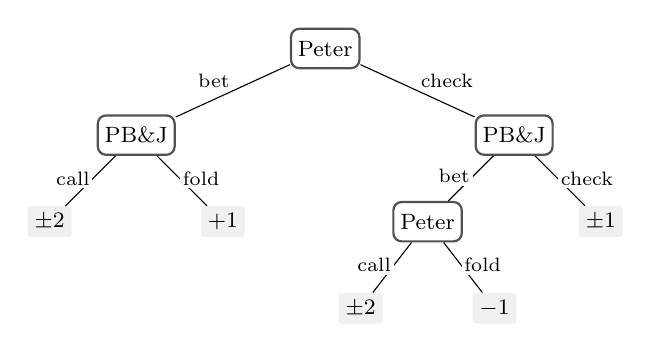
\begin{tikzpicture}[
  level distance=11mm,
  every node/.style={font=\footnotesize},
  dec/.style={rectangle, rounded corners=3pt, draw=inkmuted, thick, inner sep=2.5pt, minimum height=5mm},
  leaf/.style={rectangle, rounded corners=1pt, fill=gray!12, inner sep=2.5pt},
  lbl/.style={font=\scriptsize, fill=white, inner sep=1pt},
  level 1/.style={sibling distance=48mm},
  level 2/.style={sibling distance=22mm},
  level 3/.style={sibling distance=17mm},
]
\node[dec] {\peter}
  child { node[dec] {\pbj}
    child { node[leaf] {$\pm2$} edge from parent node[lbl, left, pos=0.45] {call} }
    child { node[leaf] {$+1$} edge from parent node[lbl, right, pos=0.45] {fold} }
    edge from parent node[lbl, above left] {bet} }
  child { node[dec] {\pbj}
    child { node[dec] {\peter}
      child { node[leaf] {$\pm2$} edge from parent node[lbl, left, pos=0.45] {call} }
      child { node[leaf] {$-1$} edge from parent node[lbl, right, pos=0.45] {fold} }
      edge from parent node[lbl, left, pos=0.45] {bet} }
    child { node[leaf] {$\pm1$} edge from parent node[lbl, right, pos=0.45] {check} }
    edge from parent node[lbl, above right] {check} };
\end{tikzpicture}
\caption{Betting tree for one hand, with \peter's net chips at each end. $\pm$
means \peter{} wins if he holds the higher card and loses otherwise.}
\label{fig:tree}
\end{figure}

\paragraph{Model.} Because \pbj{} is fixed at the equilibrium strategy, \pbj{}
becomes part of the environment, and the game is a single-agent MDP for
\peter{}. A state is \peter's information set (his card plus the betting so
far), the actions are bet/check or call/fold, and the reward is the net chips
won. Figure~\ref{fig:tree} shows the structure.

\paragraph{Assumptions and dependencies.} (1) \peter{} always acts first.
(2) \peter{} sees only his own card, so his actions depend only on that card.
(3) \pbj's actions depend only on \pbj's card and \peter's last action.
(4) The showdown outcome depends on both cards. The parameters are \peter's
four probabilities and \pbj's $q$ (fixed at $1/3$ unless stated otherwise).

\paragraph{Exact inference.} For a given strategy we compute \peter's exact EV
per hand. We add up payoff $\times$ probability over all six deals and every
branch of Figure~\ref{fig:tree}. Every coin flip is replaced by its
probability, so the result has no sampling noise. We use this exact EV as the
objective instead of a mean-squared error.

\paragraph{Learning.} We use coordinate hill climbing, a simple form of policy
search. Starting from random values of the four probabilities, we nudge each
one up or down by $\code{lr} = 0.005$ and keep the change only if it strictly
raises the EV. We repeat until no nudge helps, or for at most 1000 sweeps.

\paragraph{Approximate inference (verification).} We then estimate the same EV
by Monte Carlo sampling. We simulate $M = 200{,}000$ hands with the learned
probabilities and compare the result with the exact EV and with $-1/18$.

\paragraph{How this differed from our plan.} Our proposal planned Q-learning
agents scored by \emph{exploitability}, the amount a perfect opponent could win
against a strategy. We built something simpler: a fixed equilibrium opponent,
an exact EV objective and hill climbing. We use exploitability only to analyze
the results (Section~\ref{sec:qual}).

% ===========================================================================
\section{Results and Discussion}

\subsection{Comparing configurations}

\begin{table}[tb]
\centering
\small
\caption{Configurations compared. Learning-rate and $q$ rows use 1{,}000
random starts each; $M$ rows use repeated simulations of one equilibrium
strategy ($\alpha = 0.2$). EV is \peter's exact EV after hill climbing.}
\label{tab:configs}
\begin{tabular}{llll}
\toprule
Setting & Final EV & Learned strategy & Cost / stability \\
\midrule
\multicolumn{4}{l}{\emph{Learning rate} (\pbj{} optimal, $q = 1/3$)} \\
\code{lr} $= 0.001$ & $-1/18$ (all runs) & \code{bet\_Q} $= 0$ & 4{,}035 EV evaluations/run \\
\code{lr} $= 0.005$ (ours) & $-1/18$ (all runs) & \code{bet\_Q} $= 0$ & 822 \\
\code{lr} $= 0.02$ & $-1/18$ (all runs) & \code{bet\_Q} $= 0$ & 214 \\
\code{lr} $= 0.1$ & $-1/18$ (all runs) & \code{bet\_Q} $= 0$ & 54 \\
\midrule
\multicolumn{4}{l}{\emph{\pbj's strategy $q$} (\code{lr} $= 0.005$)} \\
$q = 0$   & $+1/6$  & \code{bet\_J}$=1$, \code{call\_Q}$=0$ & all runs agree \\
$q = 0.2$ & $+1/30$ & \code{bet\_J}$=1$, \code{call\_Q}$=0$ & all runs agree \\
$q = 1/3$ (optimal) & $-1/18$ & only \code{bet\_Q}$=0$ & 3 of 4 stay random \\
$q = 0.5$ & $0$ & \code{bet\_J}$=0$, \code{call\_Q}$=1$ & all runs agree \\
$q = 1$   & $+1/6$ or $0$ & \code{bet\_J}$=0$ & 13.5\% stuck at $0$ \\
\midrule
\multicolumn{4}{l}{\emph{Simulated hands $M$} (RMS error of simulated EV)} \\
$M = 10^3$ & $0.039$ & --- & 0.3\,ms/run \\
$M = 10^4$ & $0.013$ & --- & 3\,ms/run \\
$M = 10^5$ & $0.0037$ & --- & 36\,ms/run \\
$M = 2\times10^5$ (ours) & $0.0034$ & --- & 67\,ms/run \\
\bottomrule
\end{tabular}
\end{table}

Table~\ref{tab:configs} compares three settings.

\paragraph{Learning rate.} Every learning rate reached the same answer. A
larger \code{lr} only made training faster, roughly in proportion: from about
4{,}000 EV evaluations per run at $0.001$ down to about 50 at $0.1$. The
reason is that the EV changes only through \code{bet\_Q}, and in a straight
line (Section~\ref{sec:quant}), so step size affects speed but not the result.

\paragraph{\pbj's strategy $q$.} This was the most informative comparison.
When \pbj{} deviates from $q = 1/3$, \peter{} learns to exploit it and wins
chips. With $q$ too low (\pbj{} bluffs and calls too rarely), \peter{} always
bluffs with a Jack and never calls with a Queen. With $q$ too high, he does the
reverse. Only at $q = 1/3$ is \peter{} held to his lowest EV, $-1/18$, which
confirms that $q = 1/3$ is \pbj's optimal strategy. \code{bet\_K} stayed random
for every $q$. \pbj{} calls with a Queen exactly as often as it bluffs with a
Jack (both $q$), so \peter's King earns the same whether he bets or checks. At
$q = 1$, 13.5\% of runs got stuck at an EV of $0$ instead of $1/6$. These runs
always bet the Queen and had a low \code{call\_Q}. Checking a Queen only pays
off if \peter{} then calls, so lowering \code{bet\_Q} alone made things worse.
Raising \code{call\_Q} alone changed nothing, because \peter{} never checked a
Queen. Changing one variable at a time cannot escape this local optimum.

\paragraph{Simulated hands $M$.} The simulation error shrinks like
$1/\sqrt{M}$, so ten times more hands buys about three times more accuracy.
Our $M = 200{,}000$ gives errors of about $0.003$ per run.

\subsection{Quantitative results}
\label{sec:quant}

All 10{,}000 logged runs reached an exact EV of $-1/18$. Table~\ref{tab:indiff}
explains why. Against \pbj, \peter{} gets the same EV whatever he does, except
when he bets with a Queen. Adding up the rows gives
\[
  \text{EV} = -\frac{1 + \code{bet\_Q}}{18},
\]
so the best \peter{} can do is to set $\code{bet\_Q} = 0$, and every run
found it.

\begin{table}[htb]
\centering
\small
\caption{\peter's EV for each action, by card, against \pbj.}
\label{tab:indiff}
\setlength{\tabcolsep}{4pt}
\begin{tabular}{lccc}
\toprule
Card & If bet & If check & Share of total EV \\
\midrule
Jack  & $-1$   & $-1$   & $-1/3$ \\
Queen & $-1/2$ & $-1/3$ & $-1/9 - \code{bet\_Q}/18$ \\
King  & $7/6$  & $7/6$  & $+7/18$ \\
\midrule
Total & & & $-(1 + \code{bet\_Q})/18$ \\
\bottomrule
\end{tabular}
\end{table}

\begin{figure}[tb]
\centering
\begin{minipage}[t]{0.48\linewidth}
\centering
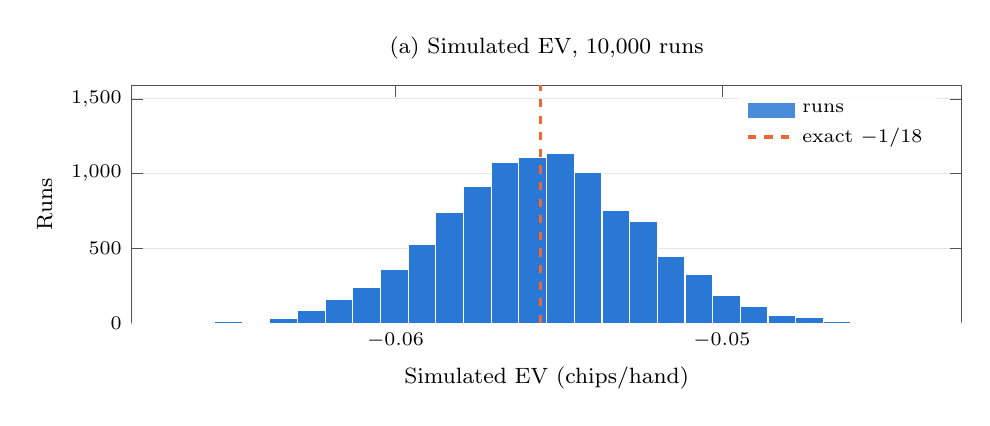
\begin{tikzpicture}[baseline=(current axis.north)]
\begin{axis}[
  width=\linewidth, height=4.6cm,
  title={(a) Simulated EV, 10{,}000 runs},
  xlabel={Simulated EV (chips/hand)}, ylabel={Runs},
  ymin=0, ymax=1590, xmin=-0.068090, xmax=-0.042650, xtick distance=0.01,
  scaled x ticks=false,
  xticklabel style={/pgf/number format/fixed, /pgf/number format/precision=2},
  legend pos=north east,
]
\addplot[ybar interval, area legend, fill=series1, draw=white, line width=0.4pt] coordinates { (-0.068090,2) (-0.067242,1) (-0.066394,2) (-0.065546,10) (-0.064698,7) (-0.063850,31) (-0.063002,84) (-0.062154,160) (-0.061306,238) (-0.060458,359) (-0.059610,526) (-0.058762,739) (-0.057914,911) (-0.057066,1073) (-0.056218,1105) (-0.055370,1136) (-0.054522,1011) (-0.053674,752) (-0.052826,683) (-0.051978,443) (-0.051130,327) (-0.050282,182) (-0.049434,110) (-0.048586,49) (-0.047738,38) (-0.046890,12) (-0.046042,5) (-0.045194,2) (-0.044346,1) (-0.043498,1) (-0.042650,1) };
\addlegendentry{runs}
\addplot[series2, very thick, dashed] coordinates {(-0.0555556,0) (-0.0555556,1590)};
\addlegendentry{exact $-1/18$}
\end{axis}
\end{tikzpicture}
\end{minipage}\hfill
\begin{minipage}[t]{0.48\linewidth}
\centering
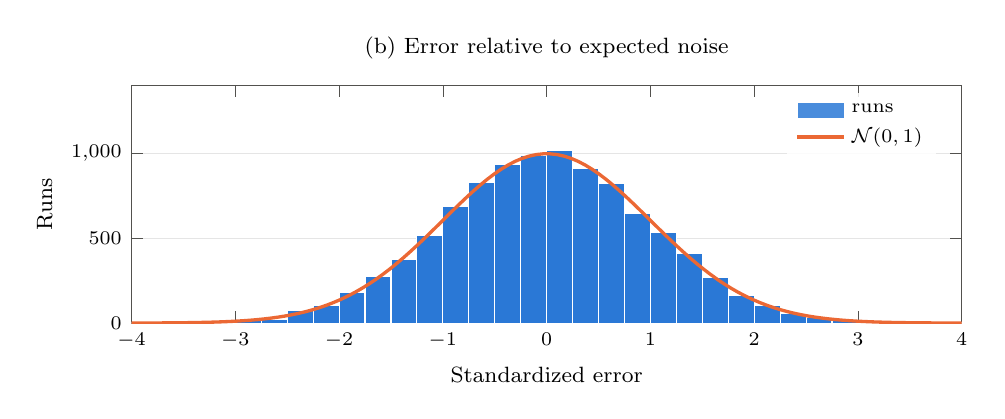
\begin{tikzpicture}[baseline=(current axis.north)]
\begin{axis}[
  width=\linewidth, height=4.6cm,
  title={(b) Error relative to expected noise},
  xlabel={Standardized error}, ylabel={Runs},
  ymin=0, ymax=1400, xmin=-4, xmax=4,
  legend pos=north east,
]
\addplot[ybar interval, area legend, fill=series1, draw=white, line width=0.4pt] coordinates { (-4.000,3) (-3.750,1) (-3.500,2) (-3.250,3) (-3.000,13) (-2.750,20) (-2.500,73) (-2.250,106) (-2.000,183) (-1.750,272) (-1.500,372) (-1.250,517) (-1.000,685) (-0.750,827) (-0.500,935) (-0.250,989) (0.000,1018) (0.250,909) (0.500,821) (0.750,645) (1.000,534) (1.250,411) (1.500,269) (1.750,161) (2.000,104) (2.250,59) (2.500,36) (2.750,17) (3.000,11) (3.250,2) (3.500,1) (3.750,1) (4.000,1) };
\addlegendentry{runs}
\addplot[series2, very thick, domain=-4:4, samples=120] {10000*0.25*exp(-x^2/2)/sqrt(2*pi)};
\addlegendentry{$\mathcal{N}(0,1)$}
\end{axis}
\end{tikzpicture}
\end{minipage}
\caption{(a) Simulated EV of all 10{,}000 runs ($M = 200{,}000$ hands each);
the dashed line is the exact value $-1/18$. (b) Each run's error divided by its
expected size, compared with a standard bell curve.}
\label{fig:sim}
\end{figure}

\begin{table}[htb]
\centering
\small
\caption{Simulated EV ($M = 200{,}000$ hands per run) compared with the exact
EV of $-1/18 = -0.0555556$, over 10{,}000 runs.}
\label{tab:dev}
\setlength{\tabcolsep}{4pt}
\begin{tabular}{lr}
\toprule
Mean simulated EV & $-0.0555564$ \\
Typical error (RMS) & $0.0030$ (5.4\%) \\
Average absolute error & $0.0024$ (4.3\%) \\
Largest error & $0.0129$ (23\%) \\
Runs within 1 / 5 / 10\% & 14.6 / 64.4 / 93.3\% \\
Runs above / below $-1/18$ & 50\% / 50\% \\
\bottomrule
\end{tabular}
\end{table}

Table~\ref{tab:dev} and Figure~\ref{fig:sim} compare the simulations with the
exact value. On average the simulation is essentially perfect: over all
$2\times10^9$ simulated hands the mean is $-0.0555564$, against a true value
of $-0.0555556$. Single runs miss by about $0.003$ (5\%), which is exactly the
error we expect from $M = 200{,}000$ random hands: each hand swings by about
$1.35$ chips, and $1.35/\sqrt{M} \approx 0.003$. When each error is divided by
its expected size, the errors follow a standard bell curve
(Figure~\ref{fig:sim}b). The gap between simulated and exact EV is therefore
just sampling noise.

\subsection{Qualitative insights}
\label{sec:qual}

\begin{figure}[tb]
\centering
\begin{minipage}[t]{0.48\linewidth}
\centering
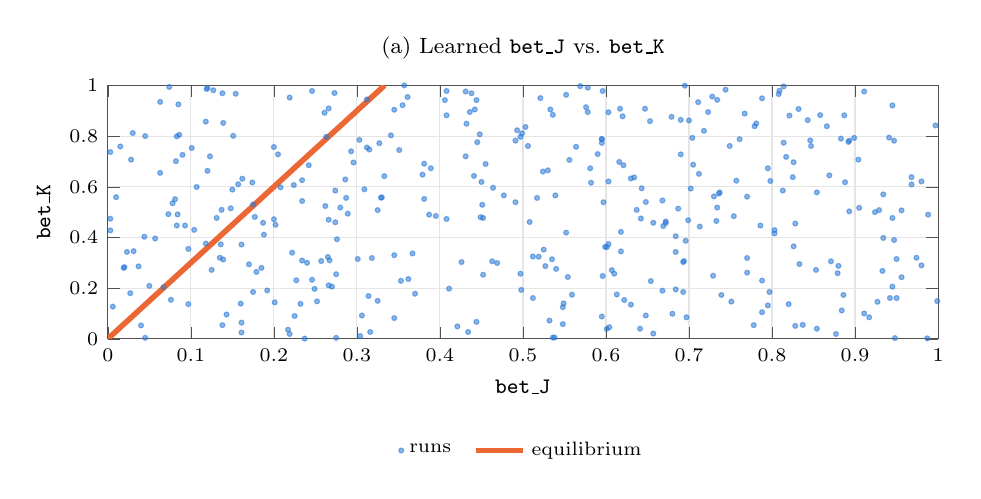
\begin{tikzpicture}[baseline=(current axis.north)]
\begin{axis}[
  width=\linewidth, height=4.8cm,
  title={(a) Learned \code{bet\_J} vs.\ \code{bet\_K}},
  legend columns=2, legend style={at={(0.5,-0.36)}, anchor=north, /tikz/every even column/.append style={column sep=6pt}},
  xlabel={\code{bet\_J}}, ylabel={\code{bet\_K}},
  xmin=0, xmax=1, ymin=0, ymax=1, xmajorgrids,
]
\addplot[only marks, mark=*, mark size=0.9pt, color=series1, fill opacity=0.55, draw opacity=0.55] coordinates { (0.444,0.942) (0.084,0.491) (0.086,0.805) (0.312,0.945) (0.293,0.74) (0.28,0.518) (0.333,0.642) (0.224,0.607) (0.175,0.185) (0.325,0.15) (0.603,0.374) (0.63,0.633) (0.536,0.884) (0.406,0.942) (0.934,0.398) (0.477,0.566) (0.452,0.477) (0.803,0.416) (0.312,0.755) (0.814,0.774) (0.77,0.261) (0.101,0.753) (0.599,0.363) (0.69,0.864) (0.927,0.146) (0.73,0.562) (0.506,0.761) (0.185,0.28) (0.669,0.445) (0.161,0.064) (0.327,0.772) (0.304,0.011) (0.647,0.908) (0.175,0.53) (0.888,0.618) (0.187,0.458) (0.61,0.257) (0.54,0.276) (0.451,0.529) (0.445,0.776) (0.286,0.629) (0.924,0.5) (0.497,0.797) (0.744,0.983) (0.781,0.85) (0.143,0.096) (0.911,0.976) (0.637,0.509) (0.843,0.863) (0.345,0.33) (0.595,0.788) (0.7,0.862) (0.974,0.32) (0.905,0.517) (0.432,0.849) (0.911,0.1) (0.107,0.599) (0.648,0.092) (0.887,0.882) (0.95,0.315) (0.361,0.954) (0.464,0.596) (0.828,0.455) (0.154,0.967) (0.123,0.72) (0.275,0.004) (0.234,0.544) (0.246,0.978) (0.968,0.638) (0.499,0.811) (0.081,0.551) (0.737,0.578) (0.438,0.969) (0.814,0.996) (0.62,0.878) (0.576,0.914) (0.085,0.925) (0.246,0.233) (0.893,0.503) (0.267,0.31) (0.234,0.309) (0.202,0.45) (0.739,0.173) (0.289,0.494) (0.693,0.303) (0.987,0.002) (0.083,0.799) (0.858,0.883) (0.718,0.821) (0.997,0.842) (0.945,0.921) (0.05,0.209) (0.668,0.19) (0.019,0.28) (0.234,0.626) (0.684,0.195) (0.788,0.949) (0.712,0.651) (0.276,0.393) (0.093,0.447) (0.98,0.29) (0.045,0.8) (0.205,0.728) (0.063,0.655) (0.88,0.288) (0.09,0.726) (0.345,0.904) (0.351,0.745) (0.734,0.943) (0.729,0.249) (0.33,0.558) (0.751,0.147) (0.696,0.387) (0.357,1.0) (0.795,0.132) (0.767,0.889) (0.797,0.185) (0.219,0.952) (0.595,0.773) (0.078,0.535) (0.728,0.956) (0.057,0.396) (0.118,0.376) (0.813,0.585) (0.578,0.895) (0.832,0.907) (0.083,0.447) (0.135,0.32) (0.552,0.963) (0.24,0.3) (0.617,0.908) (0.668,0.546) (0.803,0.429) (0.672,0.463) (0.809,0.979) (0.273,0.97) (0.455,0.69) (0.12,0.663) (0.69,0.728) (0.828,0.051) (0.521,0.95) (0.367,0.337) (0.015,0.759) (0.788,0.23) (0.266,0.47) (0.533,0.905) (0.68,0.099) (0.654,0.228) (0.503,0.836) (0.817,0.718) (0.118,0.857) (0.945,0.477) (0.067,0.204) (0.734,0.518) (0.618,0.422) (0.345,0.082) (0.934,0.57) (0.846,0.783) (0.569,0.997) (0.263,0.797) (0.657,0.021) (0.023,0.343) (0.596,0.248) (0.15,0.589) (0.641,0.04) (0.854,0.578) (0.003,0.737) (0.2,0.757) (0.217,0.036) (0.389,0.673) (0.275,0.255) (0.947,0.782) (0.01,0.559) (0.296,0.696) (0.37,0.178) (0.548,0.058) (0.262,0.524) (0.097,0.137) (0.341,0.803) (0.884,0.112) (0.879,0.259) (0.137,0.509) (0.77,0.561) (0.232,0.138) (0.441,0.643) (0.138,0.969) (0.786,0.447) (0.788,0.105) (0.833,0.295) (0.411,0.198) (0.702,0.593) (0.442,0.905) (0.265,0.323) (0.491,0.539) (0.821,0.881) (0.564,0.758) (0.082,0.701) (0.161,0.025) (0.395,0.485) (0.597,0.539) (0.266,0.211) (0.355,0.922) (0.139,0.852) (0.2,0.472) (0.222,0.34) (0.904,0.707) (0.426,0.303) (0.854,0.04) (0.705,0.687) (0.933,0.268) (0.711,0.934) (0.381,0.552) (0.653,0.859) (0.77,0.319) (0.679,0.876) (0.434,0.027) (0.274,0.585) (0.621,0.685) (0.778,0.054) (0.266,0.909) (0.325,0.508) (0.559,0.174) (0.948,0.003) (0.657,0.458) (0.723,0.895) (0.408,0.882) (0.687,0.514) (0.866,0.839) (0.512,0.161) (0.448,0.807) (0.837,0.055) (0.493,0.823) (0.554,0.244) (0.98,0.621) (0.877,0.019) (0.219,0.019) (0.188,0.411) (0.287,0.556) (0.601,0.362) (0.779,0.839) (0.03,0.812) (0.353,0.229) (0.037,0.286) (0.073,0.492) (0.548,0.125) (0.601,0.039) (0.179,0.264) (0.929,0.508) (0.883,0.79) (0.449,0.48) (0.12,0.99) (0.757,0.624) (0.53,0.665) (0.138,0.054) (0.301,0.315) (0.497,0.257) (0.463,0.306) (0.988,0.49) (0.871,0.306) (0.249,0.197) (0.362,0.236) (0.498,0.193) (0.604,0.046) (0.642,0.475) (0.148,0.515) (0.225,0.09) (0.736,0.573) (0.733,0.465) (0.556,0.706) (0.16,0.139) (0.761,0.788) (0.309,0.59) (0.192,0.191) (0.136,0.373) (0.549,0.14) (0.408,0.473) (0.693,0.185) (0.942,0.161) (0.517,0.556) (0.252,0.148) (0.028,0.707) (0.603,0.894) (0.695,0.999) (0.261,0.892) (0.968,0.609) (0.538,0.005) (0.672,0.457) (0.161,0.372) (0.613,0.175) (0.899,0.793) (0.552,0.419) (0.536,0.005) (0.003,0.428) (0.508,0.461) (0.201,0.144) (0.242,0.685) (0.684,0.405) (0.318,0.319) (0.519,0.324) (0.648,0.54) (0.524,0.66) (0.956,0.243) (0.45,0.619) (0.917,0.085) (0.27,0.206) (0.227,0.231) (0.131,0.477) (0.157,0.61) (0.097,0.355) (0.003,0.474) (0.315,0.747) (0.82,0.137) (0.795,0.673) (0.174,0.617) (0.044,0.403) (0.947,0.39) (0.17,0.294) (0.826,0.697) (0.59,0.729) (0.634,0.637) (0.006,0.127) (0.379,0.648) (0.578,0.991) (0.622,0.153) (0.853,0.272) (0.798,0.623) (0.616,0.698) (0.469,0.299) (0.491,0.782) (0.595,0.788) (0.532,0.072) (0.704,0.793) (0.314,0.169) (0.893,0.782) (0.031,0.346) (0.699,0.468) (0.208,0.598) (0.941,0.794) (0.274,0.46) (0.162,0.632) (0.125,0.272) (0.754,0.484) (0.444,0.067) (0.063,0.935) (0.316,0.027) (0.431,0.72) (0.643,0.594) (0.956,0.507) (0.945,0.206) (0.582,0.616) (0.076,0.154) (0.808,0.966) (0.749,0.761) (0.452,0.253) (0.119,0.986) (0.303,0.785) (0.713,0.443) (0.045,0.004) (0.139,0.313) (0.527,0.287) (0.421,0.049) (0.603,0.621) (0.999,0.149) (0.436,0.895) (0.408,0.978) (0.684,0.343) (0.387,0.49) (0.826,0.365) (0.151,0.801) (0.381,0.691) (0.525,0.352) (0.257,0.307) (0.306,0.092) (0.512,0.325) (0.607,0.271) (0.074,0.994) (0.63,0.135) (0.618,0.345) (0.02,0.283) (0.329,0.557) (0.847,0.761) (0.886,0.173) (0.596,0.978) (0.581,0.673) (0.104,0.43) (0.825,0.638) (0.431,0.976) (0.697,0.085) (0.04,0.053) (0.177,0.481) (0.869,0.645) (0.535,0.314) (0.127,0.981) (0.539,0.566) (0.95,0.161) (0.595,0.088) (0.694,0.307) (0.027,0.18) (0.892,0.777) (0.237,0.001) };
\addlegendentry{runs}
\addplot[series2, line width=2pt] coordinates {(0,0) (0.33333,1)};
\addlegendentry{equilibrium}
\end{axis}
\end{tikzpicture}
\end{minipage}\hfill
\begin{minipage}[t]{0.48\linewidth}
\centering
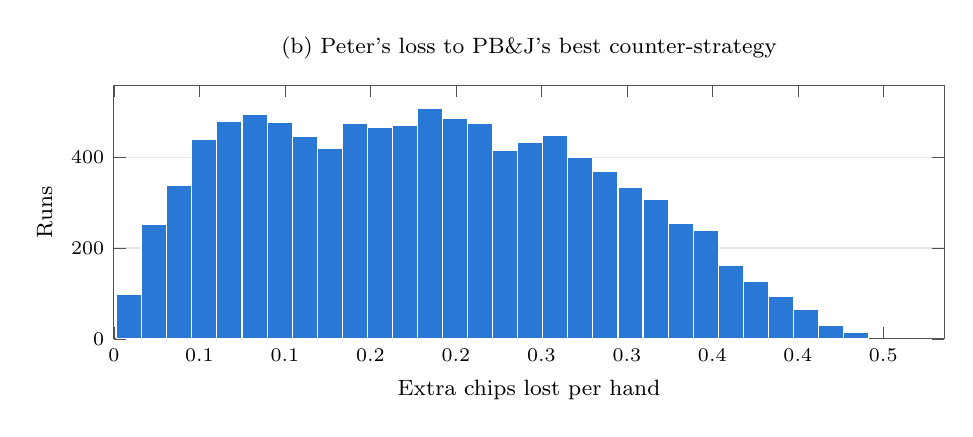
\begin{tikzpicture}[baseline=(current axis.north)]
\begin{axis}[
  width=\linewidth, height=4.8cm,
  title={(b) \peter's loss to \pbj's best counter-strategy},
  xlabel={Extra chips lost per hand}, ylabel={Runs},
  ymin=0, xmin=0,
  scaled x ticks=false,
  xticklabel style={/pgf/number format/fixed, /pgf/number format/precision=1},
]
\addplot[ybar interval, fill=series1, draw=white, line width=0.4pt] coordinates { (0.00161,98) (0.01627,251) (0.03093,337) (0.04559,439) (0.06026,479) (0.07492,494) (0.08958,477) (0.10424,445) (0.11890,420) (0.13356,475) (0.14822,465) (0.16288,469) (0.17754,507) (0.19221,485) (0.20687,474) (0.22153,414) (0.23619,432) (0.25085,448) (0.26551,399) (0.28017,368) (0.29483,334) (0.30949,307) (0.32416,253) (0.33882,238) (0.35348,162) (0.36814,127) (0.38280,94) (0.39746,65) (0.41212,30) (0.42678,14) (0.44144,14) };
\end{axis}
\end{tikzpicture}
\end{minipage}
\caption{(a) Learned \code{bet\_J} against \code{bet\_K} for 400 random runs.
At equilibrium every point would lie on the orange line
($\code{bet\_J} = \alpha$, $\code{bet\_K} = 3\alpha$). (b) How much more each
learned strategy would lose if \pbj{} switched to its best counter-strategy
(0 for an equilibrium strategy).}
\label{fig:strategy}
\end{figure}

\begin{table}[htb]
\centering
\small
\caption{\peter's learned probabilities over 10{,}000 runs, compared with the
equilibrium (Eq.~\ref{eq:equilibrium}). A uniform random number has mean
$0.5$ and SD $0.29$.}
\label{tab:params}
\begin{tabular}{lccl}
\toprule
Probability & Mean & SD & Equilibrium \\
\midrule
\code{bet\_J}  & 0.505 & 0.287 & $\alpha \in [0, 1/3]$ \\
\code{bet\_Q}  & 0.000 & 0.000 & $0$ \\
\code{bet\_K}  & 0.498 & 0.288 & $3\alpha$ \\
\code{call\_Q} & 0.501 & 0.286 & $\alpha + 1/3$ \\
\bottomrule
\end{tabular}
\end{table}

\paragraph{What the model captures.} The model captures the probabilistic
reasoning behind the equilibrium. For example, if \peter{} checks a Queen and
\pbj{} bets, \pbj{} holds the King $3/4$ of the time by Bayes' rule
($P(K \mid \text{bet}) = \frac{1 \cdot 1/2}{1 \cdot 1/2 + 1/3 \cdot 1/2}$). So
calling and folding both average $-1$ chip, which is exactly why
\code{call\_Q} does not matter against \pbj. \pbj's bluffing rate of $1/3$ is
chosen to make \peter{} indifferent in this way.

\paragraph{What the model misses.} Only \code{bet\_Q} matched the equilibrium
(Table~\ref{tab:params}). The other three probabilities look exactly like
uniform random numbers. They have no effect on the EV, so the hill climber
never accepted a change to them, and they stayed at their random starting
values. Figure~\ref{fig:strategy}a shows that \code{bet\_J} and \code{bet\_K}
are scattered across the whole square instead of lying on the equilibrium
line. Only 1.3\% of runs came within $0.1$ of an equilibrium strategy for some
$\alpha$. This matters because a real opponent would not stay fixed. If \pbj{}
switched to its best counter-strategy, it would win an extra $0.19$ chips per
hand on average from \peter's learned strategies (Figure~\ref{fig:strategy}b),
more than three times the equilibrium value itself. Our proposal expected
this when training against a fixed opponent: the learner exploits that
opponent well but can itself be exploited.

\subsection{Convergence and scalability}

Training was stable. Against the optimal \pbj, every run converged, to the
same EV, within at most 200 productive sweeps (well under the 1000-sweep cap).
The only instability we saw was the local optimum at $q = 1$
(Table~\ref{tab:configs}). Training is cheap: each exact EV evaluation is six
terms. Almost all of the cost is verification. One 200{,}000-hand simulation
takes about $0.07$\,s, so the 10{,}000-run log ($2\times10^9$ hands) took
about 11 minutes. More data, meaning more restarts or more simulated hands,
would shrink the simulation error but would not change the learned strategy,
because the gap to the equilibrium comes from the objective, not from noise.
Exact enumeration also does not scale: real poker has far too many deals and
betting sequences to add them all up, which is where sampling and learning
methods become necessary.

% ===========================================================================
\section{Conclusion}

We trained \peter{} by hill climbing on the exact EV against \pbj{} playing
the equilibrium. Every one of 10{,}000 runs reached the optimal value of
$-1/18$, and simulations of $M = 200{,}000$ hands confirmed it to within
ordinary sampling noise. Choosing variables per card instead of per deal was
what made the model correct. Against non-optimal versions of \pbj, \peter{}
learned to exploit them, which confirms that $q = 1/3$ is \pbj's optimal
strategy.

\paragraph{Limitations.} The learned strategies were not optimal. Against
\pbj, only \code{bet\_Q} affects the EV, so \code{bet\_J}, \code{bet\_K} and
\code{call\_Q} stayed wherever they started, and a smarter opponent could
exploit them. Changing one variable at a time can also get stuck at local
optima.

\paragraph{Extensions.} To learn the full equilibrium, the objective has to
account for an opponent who adapts. Possible next steps are to minimize
exploitability directly, to let both players learn as originally proposed,
and to move on to three-player Kuhn poker~\cite{wiki,szafron2013}. Our model
got the right answer for the value while mostly missing the strategy behind
it. As the professor says: all models are wrong but some are useful.

% ===========================================================================
\section{Reflections \& Contributions}

\paragraph{Advice for future students.} Check early that every variable in
your model only uses information the agent can actually see; our first
six-variable design did not, and it skewed every result. Compute exact answers
whenever the problem is small enough, and use simulation as a check rather
than the main tool. Finally, matching the right \emph{number} does not mean the
model learned the right \emph{behavior}, so look at the learned parameters, not
just the score.

\paragraph{Contributions and individual reflections.}
\begin{itemize}\itemsep2pt
  \item \textbf{Shawn Wang:} [1--2 sentences on tasks]. \emph{Reflection:} [what you learned].
  \item \textbf{David Yu:} [1--2 sentences on tasks]. \emph{Reflection:} [what you learned].
  \item \textbf{Kevin Pyo:} [1--2 sentences on tasks]. \emph{Reflection:} [what you learned].
  \item \textbf{Brian Gasca:} [1--2 sentences on tasks]. \emph{Reflection:} [what you learned].
  \item \textbf{Daniel Wu:} [1--2 sentences on tasks]. \emph{Reflection:} [what you learned].
\end{itemize}

\paragraph{Use of generative AI.} 
% What you guys feel
% We used Claude to help draft and format this report in LaTeX and to run the additional configuration experiments in Table~\ref{tab:configs} with our own \code{logic.py} functions. All modeling decisions, code and final content were reviewed and verified by the team.


% ===========================================================================
\section{References}
{\renewcommand{\section}[2]{}%
\begin{thebibliography}{9}
\small
\bibitem{wiki}
``Kuhn poker,'' \emph{Wikipedia}.
\url{https://en.wikipedia.org/wiki/Kuhn_poker}

\bibitem{kuhn1950}
H.~W. Kuhn, ``Simplified two-person poker,'' in H.~W. Kuhn and A.~W. Tucker
(eds.), \emph{Contributions to the Theory of Games}, vol.~1, Princeton
University Press, 1950, pp.~97--103. (Cited by~\cite{wiki}.)

\bibitem{szafron2013}
D.~Szafron, R.~Gibson, and N.~Sturtevant, ``A parameterized family of
equilibrium profiles for three-player Kuhn poker,'' in \emph{Proc.\ 12th Int.\
Conf.\ on Autonomous Agents and Multiagent Systems (AAMAS)}, 2013. (Cited
by~\cite{wiki}.)
\end{thebibliography}}

\end{document}